\section{Исследовательский раздел \hfill}
\vspace{\baselineskip}


\subsection{Технические характеристики}

Технические характеристики устройства, на котором выполнялись замеры времени:

\begin{itemize}[label=---]
	\item операционная система Windows 10;
	\item память 8 ГБ;
	\item процессор Intel® Core™ i5-6260U @ 1.80 ГГц.
\end{itemize}

Замеры времени выполнения реализаций алгоритмов проводились на ноутбуке, включенном в сеть электропитания. Во время тестирования ноутбук был нагружен только встроенными приложениями окружения, а также непосредственно разработанным приложением.

\subsection{Демонстрация работы программы}

На рисунке \ref{fig:output} представлен пример работы программы. Пользователь вводит размеры и значения каждой из двух матриц. Программа выводит на экран результат умножения, вычисленный с помощью каждого из рассматриваемых алгоритмов.
\clearpage

\begin{figure}[h!btp]
	\centering
	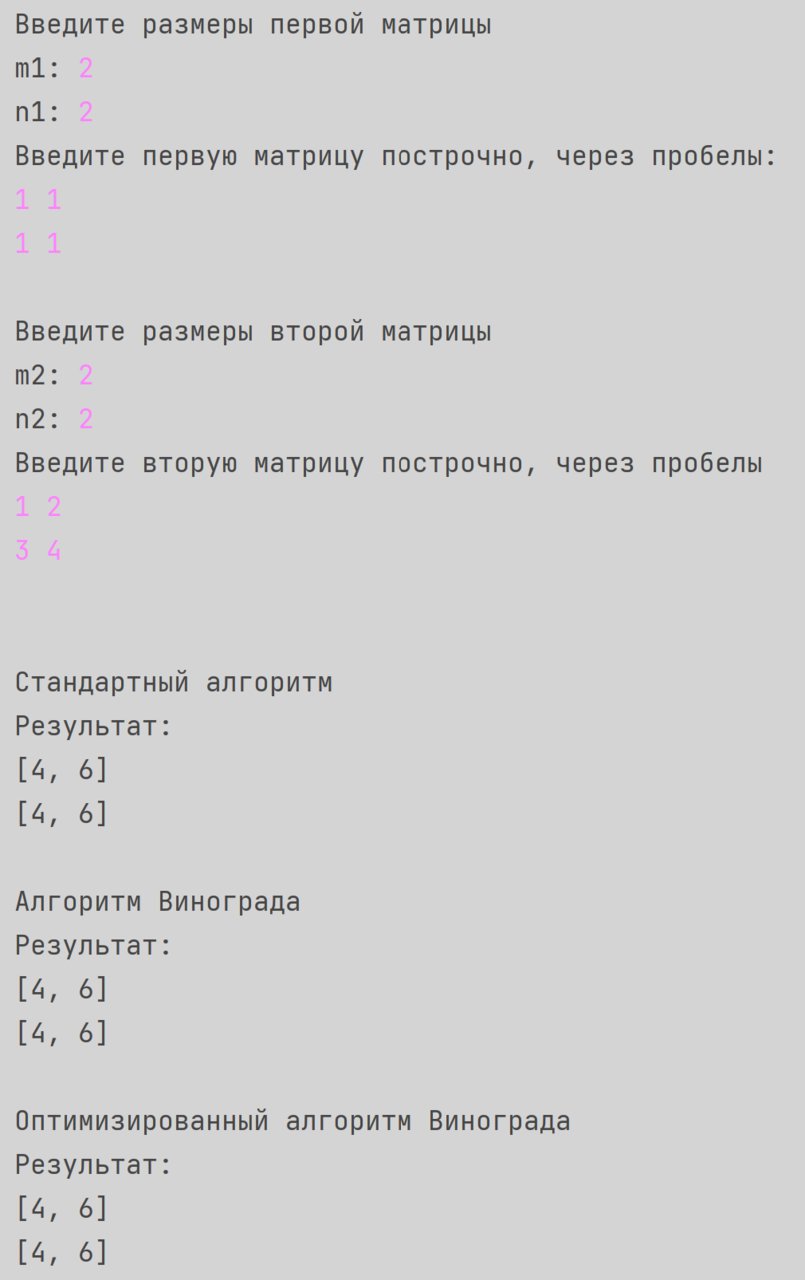
\includegraphics[width=250pt]{inc/output.png}
	\caption{Пример работы программы}
	\label{fig:output}	
\end{figure}

\subsection{Сравнение времени выполнения реализаций алгоритмов}

 Все реализации алгоритмов сравнивались на случайно сгенерированных квадратных матрицах размерностями n\cdot n, где n изменялось от 100 до 1000 с шагом 100 (лучший случай) и от 101 до 1001 с шагом 100 (худший случай).
 
На рисунке \ref{fig:plots-best} приведены результаты сравнения времени работы всех реализаций на лучшем случае (четная размерность), а на рисунке \ref{fig:plots-worst} --- на худшем (нечетная). 

\clearpage

\begin{figure}[h!btp]
	\centering
	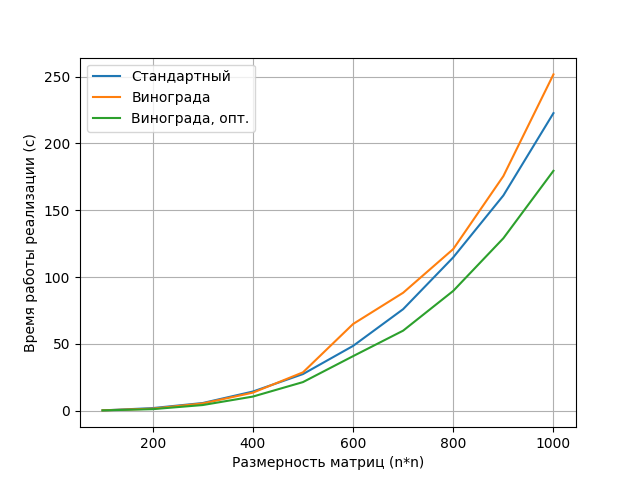
\includegraphics[width=360pt]{inc/plots-best.png}
	\caption{Сравнение времени работы реализаций алгоритмов (л.с.)}
	\label{fig:plots-best}	
\end{figure}

\begin{figure}[h!btp]
	\centering
	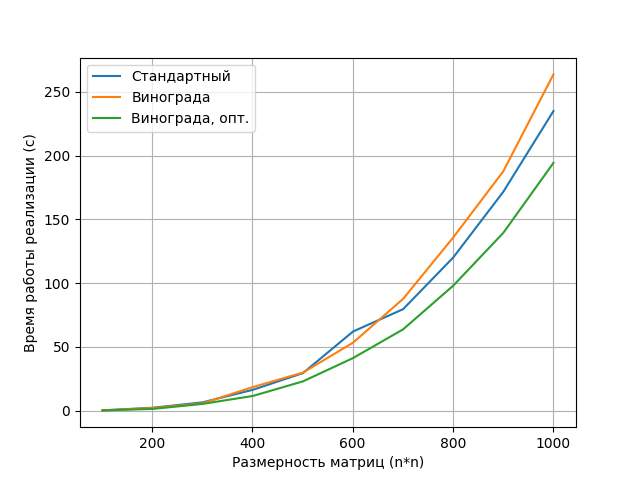
\includegraphics[width=360pt]{inc/plots-worst.png}
	\caption{Сравнение времени работы реализаций алгоритмов (х.с.)}
	\label{fig:plots-worst}	
\end{figure}


\clearpage
\subsection*{Вывод}
Были подтверждены теоретические расчеты: все алгоритмы кубически зависят от размерностей матриц. При этом реализация алгоритма Винограда работает дольше реализации стандартного алгоритма, а реализация алгоритма Винограда с оптимизациями -- быстрее.
 
Таким образом, несмотря на сложность алгоритма Винограда по сравнению со стандартным, меньшая доля умножений в нем при применении оптимизаций позволяет получить меньшую трудоемкость.